\chapter{Thực nghiệm và đánh giá}
\label{chap:chap5}
\section{Đánh giá chất lượng dữ liệu}

Để đảm bảo và theo dõi chất lượng của bộ dữ liệu trong suốt vòng đời nghiên cứu, chúng tôi đã thiết lập một quy trình đánh giá định kỳ. Quy trình này được thực hiện tại hai thời điểm then chốt: trước và sau giai đoạn tiền xử lý dữ liệu. Khung đánh giá của chúng tôi tập trung vào bốn khía cạnh cốt lõi, được đo lường thông qua các chỉ số trực tiếp và gián tiếp. Các chỉ số này bao gồm: \textbf{tính đầy đủ} (completeness), \textbf{tính nhất quán} (consistency), \textbf{mức độ liên quan} (relevance) và \textbf{độ tin cậy} (reliability). 

\textbf{Completeness}\cite{nguyen2025data} thể hiện mức độ mà các thông tin cần thiết đã được ghi nhận đầy đủ trong tập dữ liệu, không bị khuyết thiếu. Một tập dữ liệu được xem là đạt tiêu chuẩn về tính đầy đủ khi các thuộc tính chứa giá trị hợp lệ ở mỗi bản ghi. Cách đo như sau: 

\begin{equation}
\text{Completeness}_{object} = \frac{|\{ a_i \in A \mid a_i \neq \text{NaN} \land a_i \neq \text{None} \}|}{|A|} \times 100
\end{equation}
\begin{equation}
\text{Completeness}_{dataset} = \frac{1}{N} \sum_{j=1}^{N} \text{Completeness}_{object_j}
\end{equation}
Trong đó, $A = \{a_1, a_2, \ldots, a_n\}$ là tập các thuộc tính của một đối tượng, $a_i$ là giá trị của thuộc tính thứ $i$, $|A|$ là tổng số thuộc tính, và tử số là số lượng thuộc tính có giá trị không bị thiếu.

Chỉ số này giúp xác định tỷ lệ dữ liệu có sẵn so với tổng số giá trị kỳ vọng. Việc đảm bảo tính đầy đủ là mục tiêu quan trọng trong giai đoạn tiền xử lý dữ liệu.


\textbf{Consistency} \cite{nguyen2025data} đánh giá mức độ mà các giá trị trong tập dữ liệu tuân thủ các quy tắc hoặc ràng buộc logic đã được định nghĩa trước. Đây là một tiêu chí quan trọng để đảm bảo rằng dữ liệu không chứa các sai sót mang tính logic hoặc mâu thuẫn nội tại giữa các trường thông tin. Cách đo như sau:

\begin{equation}
\text{Consistency}_{object} = \frac{|\{ c_j \in C \mid isValid(c_j) = \text{True} \}|}{|C|}
\end{equation}

\begin{equation}
\text{Consistency}_{dataset} = \frac{1}{N} \sum_{j=1}^{N} \text{Consistency}_{object_j}
\end{equation}

Trong đó, $C = \{c_1, c_2, \ldots, c_m\}$ là tập các điều kiện kiểm tra áp dụng cho một đối tượng, $isValid(c_j)$ là hàm đánh giá xem điều kiện $c_j$ có được thỏa mãn hay không, và $|C|$ là tổng số điều kiện kiểm tra.

Tính nhất quán của tập dữ liệu được đánh giá dựa trên một loạt điều kiện kiểm tra được định nghĩa trước, phản ánh các quy tắc về cấu trúc và ngữ nghĩa, bao gồm:

\begin{itemize}
    \item \textbf{Ràng buộc miền giá trị (Domain range):} $a_i \in [v_{\text{min}}, v_{\text{max}}]$
    \item \textbf{Không rỗng (Non-null):} $a_i \neq \text{null}$
    \item \textbf{Kiểu dữ liệu (Data type):} $a_i \in \text{type}(a_i)$
    \item \textbf{Ràng buộc logic (Logical constraints):} ví dụ $a_i > a_j$
    \item \textbf{Tính duy nhất (Uniqueness):} $a_i \notin \text{duplicates}(A)$
    \item \textbf{Toàn vẹn khóa ngoại (Foreign key integrity):} $a_i \in \text{ReferenceTable}$
\end{itemize}

Các quy tắc kiểm tra này đóng vai trò nền tảng để tính toán chỉ số nhất quán và hỗ trợ phát hiện các vi phạm ngữ nghĩa trong tập dữ liệu. \textbf{Các nhóm trường dữ liệu được kiểm tra và quy tắc áp dụng:}

\begin{itemize}
    \item[(a)] \textbf{Các trường định danh và phân loại:}
    \begin{itemize}
        \item \texttt{user\_id}, \texttt{course\_id}, \texttt{school}: không được thiếu (\texttt{null}) và phải đúng kiểu \texttt{object}.
        \item \texttt{gender}: chỉ nhận các giá trị \{0, 1, 2\} hoặc để trống.
        \item \texttt{enroll\_time}: phải có định dạng ngày giờ hợp lệ.
        \item \texttt{classification}: chỉ chấp nhận các giá trị thuộc tập \{A, B, C, D, E\}.
    \end{itemize}

    \item[(b)] \textbf{Các trường hành vi theo tuần (Tuần 1–4):}
    \begin{itemize}
        \item \texttt{comment\_count\_week\{n\}}, \texttt{reply\_count\_week\{n\}}: là số nguyên không âm.
        \item \texttt{questions\_done\_week\{n\}}: $\geq 0$.
        \item \texttt{attempts\_count\_week\{n\}}: $\geq$ \texttt{questions\_done\_week\{n\}}.
        \item \texttt{correct\_answers\_week\{n\}}: $\leq$ \texttt{questions\_done\_week\{n\}}.
        \item \texttt{total\_score\_week\{n\}}: $\geq 0$.
        \item \texttt{user\_watching\_time\_week\{n\}}: $\geq 0$.
    \end{itemize}

    \item[(c)] \textbf{Kiểm tra toàn bộ bản ghi:}
    \begin{itemize}
        \item Kiểm tra tính \textit{duy nhất} của từng bản ghi bằng cách phát hiện các dòng trùng lặp hoàn toàn.
    \end{itemize}
\end{itemize}

\textbf{Kết quả đầu ra:} Sau khi kiểm tra, hệ thống trả về:
\begin{itemize}
    \item Tỷ lệ bản ghi hoàn toàn hợp lệ (\textit{record-level consistency}).
    \item Tỷ lệ ô dữ liệu hợp lệ (\textit{cell-level consistency}).
    \item Tỷ lệ trung bình theo trường dữ liệu (\textit{object-level consistency}).
    \item Danh sách các quy tắc bị vi phạm nhiều nhất để phục vụ phân tích nguyên nhân.
\end{itemize}

Kiểm tra tính nhất quán cho phép nhận diện các sai lệch trong hành vi học tập, lỗi về định dạng hoặc các mâu thuẫn giữa các trường dữ liệu. 

\textbf{Reliability (Độ tin cậy):} Chỉ số này đo lường sự ổn định và nhất quán của các kết quả dự đoán mà một mô hình học máy có thể tạo ra từ một bộ dữ liệu nhất định. Trong lĩnh vực phân tích dữ liệu học tập, độ tin cậy thể hiện liệu rằng bộ dữ liệu đầu vào có đủ tốt để các mô hình khác nhau, hoặc cùng một mô hình qua các lần huấn luyện khác nhau, đều đưa ra những kết luận dự báo tương tự nhau hay không. Vì đây là một thuộc tính gián tiếp, không thể đo lường trực tiếp như các thuộc tính cấu trúc (độ đầy đủ, độ nhất quán), chúng tôi đánh giá nó thông qua hiệu năng dự đoán của mô hình. Cụ thể, hai chỉ số phổ biến là F1-score và Accuracy được sử dụng làm thước đo đại diện\cite{zhang2019reliability}.  


\textbf{Relevance}: Mức độ liên quan phản ánh khả năng của các thuộc tính trong tập dữ liệu đóng góp vào việc giải thích hoặc dự đoán biến mục tiêu. Một thuộc tính được xem là có tính liên quan cao nếu nó mang lại thông tin hữu ích cho mô hình, giúp mô hình phân biệt rõ ràng giữa các lớp nhãn.

Khác với các tiêu chí như tính đầy đủ (Completeness) hay tính nhất quán (Consistency), mức độ liên quan (Relevance) mang tính trừu tượng và không thể đánh giá trực tiếp từ dữ liệu thô. Vì vậy, trong nghiên cứu này, chúng tôi sử dụng phương pháp gián tiếp để đo lường Relevance, thông qua chỉ số AUC-ROC (Area Under the Receiver Operating Characteristic Curve), nhằm phản ánh khả năng phân biệt giữa các nhãn đầu ra của mô hình trên cơ sở dữ liệu đã xử lý.
\begin{itemize}
    \item \textbf{AUC-ROC:} Là chỉ số đo diện tích dưới đường cong ROC, biểu thị mức độ mà mô hình có thể phân biệt chính xác giữa các lớp. Giá trị AUC càng lớn cho thấy dữ liệu đầu vào càng giàu thông tin và được tính toán theo công thức:

    \begin{equation}
        \text{AUC} = \int_{0}^{1} TPR(FPR^{-1}(x)) \, dx
    \end{equation}

    Trong đó:
    \begin{itemize}
        \item \textbf{TPR (True Positive Rate)} = $\frac{TP}{TP + FN}$
        \item \textbf{FPR (False Positive Rate)} = $\frac{FP}{FP + TN}$
    \end{itemize}
\end{itemize}

Dữ liệu có mức độ liên quan (Relevance) cao thường cho phép mô hình đạt AUC-ROC gần 1.0, cho thấy khả năng phân biệt giữa các lớp rất tốt. Ngược lại, nếu dữ liệu thiếu thông tin quan trọng hoặc nhiễu, AUC sẽ tiệm cận 0.5, tương đương với việc mô hình dự đoán ngẫu nhiên. Vì vậy, việc nâng cao độ liên quan thông qua các kỹ thuật như chọn lọc đặc trưng (feature selection), xây dựng đặc trưng mới (feature engineering), hoặc tích hợp thêm dữ liệu có giá trị là điều thiết yếu. 

\section{Tiêu chí đánh giá hiệu suất mô hình}
 Nhằm phản ánh chính xác mức độ cân bằng giữa các lớp và mang lại góc nhìn đánh giá khách quan và toàn diện hơn, ngoài các độ đo cơ bản như \textbf{Precision}, \textbf{Recall} và \textbf{F1-Score}, nghiên cứu này còn kết hợp sử dụng hai phương pháp tính trung bình: \textbf{macro average} và \textbf{weighted average}.

\begin{itemize}
    \item \textbf{Macro Average:} Tính trung bình F1-score trên tất cả các lớp, mà không quan tâm đến kích thước (số lượng mẫu) của từng lớp. Điều này đảm bảo rằng các lớp hiếm không bị “lấn át” bởi các lớp phổ biến.
    \begin{equation}
        \text{F1}_{\text{macro}} = \frac{1}{N} \sum_{i=1}^{N} \text{F1}_i
    \end{equation}
    Trong đó $N$ là số lớp, và $\text{F1}_i$ là F1-score của lớp thứ $i$.

    \item \textbf{Weighted Average:} Tính trung bình F1-score theo trọng số của từng lớp, với trọng số là tỷ lệ xuất hiện của lớp đó trong tập dữ liệu. Cách tính này phản ánh chính xác hơn hiệu suất mô hình trong toàn bộ tập mẫu.
    \begin{equation}
        \text{F1}_{\text{weighted}} = \sum_{i=1}^{N} w_i \times \text{F1}_i
    \end{equation}
    Với $w_i = \frac{n_i}{\sum_j n_j}$ là tỷ lệ mẫu thuộc lớp $i$ trên toàn bộ tập dữ liệu.
\end{itemize}

\textbf{Ý nghĩa:} 
\begin{itemize}
    \item F1-macro cho biết hiệu suất đồng đều của mô hình giữa các lớp.
    \item F1-weighted cho biết hiệu suất tổng thể có tính đến phân bố lớp.
\end{itemize}

\textbf{Ứng dụng:} Việc tính toán đồng thời F1-macro và F1-weighted cho mỗi mô hình học máy đảm bảo việc đánh giá hiệu suất là toàn diện và công bằng với tất cả các lớp. Các chỉ số này phản ánh khả năng mô hình mở rộng và thích ứng trong các tình huống thực tế. Điều này đặc biệt có ý nghĩa đối với các lớp dữ liệu thiểu số, chẳng hạn như nhóm người học có kết quả thấp.
\section{Phương pháp thực nghiệm}
\begin{table}[!htbp]
\centering
\caption{Preprocessing Strategies and Baseline Models}
\label{tab:baseline-models}
\scriptsize
\renewcommand{\arraystretch}{1.2}
\setlength{\tabcolsep}{1pt}
\resizebox{\columnwidth}{!}{%
\begin{tabular}{|c|c|c|c|c|c|c|c|c|c|c|c|}
    \hline
    \multirow{2}{*}{} & \multicolumn{7}{c|}{\textbf{Preprocessing}} & \multicolumn{4}{c|}{\textbf{Model}} \\ 
    \cline{2-12}
    & Raw & LD & Mean & Median & KNN & KI & GCN & LSTM & GRU & RNN & BiLSTM \\ 
    \hline
    Zero-1     & \checkmark &        &       &        &       &     &      & \checkmark & \checkmark & \checkmark & \checkmark \\ 
    \hline
    Drop-2     &            & \checkmark &   &        &       &     &      & \checkmark & \checkmark & \checkmark & \checkmark \\ 
    \hline
    Mean-3     &            &        & \checkmark &   &       &     &      & \checkmark & \checkmark & \checkmark & \checkmark \\ 
    \hline
    Median-4   &            &        &       & \checkmark &   &     &      & \checkmark & \checkmark & \checkmark & \checkmark \\ 
    \hline
    KNN-5      &            &        &       &        & \checkmark &  &      & \checkmark & \checkmark & \checkmark & \checkmark \\ 
    \hline
    KI-6       &            &        &       &        &        & \checkmark &  & \checkmark & \checkmark & \checkmark & \checkmark \\
    \hline
    \textbf{GCN-I} &        &        &       &        &       &     & \checkmark & \checkmark & \checkmark & \checkmark & \checkmark \\ 
    \hline
\end{tabular}
}
\vspace{0.5em}
\raggedright \scriptsize
\textit{Note: LD = Listwise Deletion.}
\end{table}
Để đánh giá một cách định lượng hiệu quả của phương pháp GCN-I, một phân tích so sánh đã được thực hiện. Phương pháp của chúng tôi được đối chiếu với năm kỹ thuật xử lý dữ liệu thiếu phổ biến, được xem như các mô hình cơ sở (baseline models). Tất cả các kỹ thuật này đều được áp dụng ở giai đoạn tiền xử lý, trước khi đưa dữ liệu vào huấn luyện các mô hình học sâu. Dưới đây là mô tả chi tiết về từng phương pháp cơ sở:

\begin{itemize}
    \item \textbf{Zero-1 (Điền khuyết bằng hằng số 0):} Đây là một kỹ thuật điền khuyết đơn biến, trong đó mọi giá trị bị thiếu trong tập dữ liệu đều được gán bằng hằng số 0. Mặc dù đơn giản, phương pháp này có thể làm sai lệch phân phối dữ liệu gốc.

    \item \textbf{Drop-2 (Loại bỏ hàng theo ngưỡng):} Kỹ thuật này thực hiện việc loại bỏ hàng (casewise deletion) dựa trên một ngưỡng định trước. Cụ thể, các quan sát có tỷ lệ thiếu hụt từ 50\% trở lên sẽ bị loại khỏi tập dữ liệu nhằm giữ lại các bản ghi có độ toàn vẹn thông tin cao hơn.

    \item \textbf{Mean-3 (Điền khuyết bằng giá trị trung bình):} Mỗi thuộc tính có giá trị thiếu được điền bằng giá trị trung bình (mean) của chính thuộc tính đó, được tính toán từ các giá trị hợp lệ còn lại.

    \item \textbf{Median-4 (Điền bằng trung vị):} Thay thế các giá trị thiếu bằng trung vị của từng thuộc tính, giúp giảm ảnh hưởng từ các giá trị cực đoan trong dữ liệu lệch.

    \item \textbf{KNN-5 (Điền bằng K láng giềng gần nhất):} Sử dụng thuật toán KNN để ước lượng giá trị thiếu dựa trên các bản ghi tương đồng về đặc trưng, nhằm tạo ra giá trị điền khuyết sát với thực tế hơn.
\end{itemize}

Sau khi áp dụng từng kỹ thuật điền khuyết, bốn mô hình học sâu phổ biến: RNN, GRU, BiLSTM và 4-layer-stacked LSTM sử dụng dữ liệu để huấn luyện. Cách tiếp cận này cho phép đánh giá không chỉ hiệu quả riêng biệt của từng phương pháp xử lý dữ liệu, mà còn làm rõ mức độ tương thích của các mô hình khác nhau.
% \begin{itemize}
%     \item \textbf{RNN (Recurrent Neural Network):} Mạng nơ-ron hồi tiếp cơ bản, có khả năng ghi nhớ thông tin từ các bước thời gian trước. Tuy nhiên, mô hình này dễ gặp vấn đề mất/khuyếch đại gradient khi xử lý chuỗi dài.

%     \item \textbf{LSTM (Long Short-Term Memory):} Khắc phục hạn chế của RNN bằng cơ chế cổng, cho phép lưu trữ và quên thông tin một cách có kiểm soát. LSTM phù hợp để học các phụ thuộc dài hạn.

%     \item \textbf{GRU (Gated Recurrent Unit):} Phiên bản đơn giản hơn của LSTM với ít tham số hơn, giúp giảm thời gian huấn luyện trong khi vẫn duy trì hiệu quả xử lý chuỗi.

%     \item \textbf{BiLSTM (Bidirectional LSTM):} Kết hợp hai LSTM theo hai hướng ngược nhau, giúp khai thác thông tin từ cả quá khứ và tương lai của chuỗi dữ liệu, nâng cao độ chính xác trong dự đoán.
% \end{itemize}
\section{Kết quả thực nghiệm}
\subsection{Câu hỏi nghiên cứu}
Nghiên cứu này đặt ra các câu hỏi cốt lõi như sau:

\begin{enumerate}[(i)]
\item Liệu \textbf{GCN-I} có mang lại sự cải thiện về chất lượng dữ liệu đầu vào so với các kỹ thuật điền khuyết truyền thống như \textit{Mean}, \textit{Median} hoặc \textit{Listwise Deletion}?
\item Việc áp dụng \textbf{GCN-I} ảnh hưởng ra sao đến hiệu suất của các mô hình học máy đối với các lớp ít xuất hiện như nhãn \textbf{D}?
\end{enumerate}
\subsection{Chất lượng dữ liệu}
\renewcommand\arraystretch{2.8}
\begin{sidewaystable} 
\centering
\normalsize
\caption{So sánh hiệu quả của các phương pháp điền khuyết đối với chất lượng dữ liệu}
\label{tab:results-table-quality}
\resizebox{\textheight}{!}{ % Mở rộng bảng theo chiều cao giấy
    \begin{tabular}{|c|c|c|c|c|c|c|c|c|c|c|c|c|c|c|c|c|c|c|c|c|c|c|}
        \hline
        \multirow{4}{*}{\textbf{Dataset}} & \multicolumn{2}{c|}{\textbf{Direct Evaluation}} & \multicolumn{20}{c|}{\textbf{Indirect Evaluation}} \\
        \cline{2-23}
        & \multirow{2}{*}{\textbf{Completeness}} & \multirow{2}{*}{\textbf{Consistency}} & \multicolumn{12}{c|}{\textbf{Reliability}} & \multicolumn{8}{c|}{\textbf{Relevance}}\\
        \cline{4-23}
        & & &\multicolumn{4}{c|}{Accuracy} & \multicolumn{8}{c|}{F1-Score} & \multicolumn{8}{c|}{AUC-ROC} \\
        \cline{4-23}
        & & & \multirow{2}{*} {RNN} & \multirow{2}{*} {LSTM} & \multirow{2}{*} {BiLSTM} & \multirow{2}{*} {GRU} & \multicolumn{4}{c|}{Label D} & \multicolumn{4}{c|}{Label E} & \multicolumn{4}{c|}{Label D} & \multicolumn{4}{c|}{Label E}\\ 
        \cline{8-23}
        & & & &  & & & RNN & LSTM & BiLSTM & GRU & RNN & LSTM & BiLSTM & GRU & RNN & LSTM & BiLSTM & GRU & RNN & LSTM & BiLSTM & GRU \\
        \cline{7-23}
       
        \hline
        Raw data & 39.38\% & 77.57\% & 0.65 & 0.71 & 0.72 & 0.81 & 0.52 & 0.60 & 0.56 & 0.72 & 0.78 & 0.85 & 0.84 & 0.91 & 0.87 & 0.88 & 0.90 & 0.94 & 0.88 & 0.86 & 0.91 & 0.97 \\
        \hline
        Listwise Deletion & 100\% & 100\% & 0.57  & 0.64 & 0.67 & 0.57 & 0.55 & 0.54 & 0.57 & 0.54 & 0.66 & 0.75 & 0.77 & 0.63 & 0.85 & 0.83 & 0.83 & 0.85 & 0.81 & 0.87 & 0.84 & 0.84      \\
        \hline
        Mean & 100\% & 100\% & 0.91 & 0.85 & 0.90 & 0.75 & 0.55 & 0.36 & 0.49 & 0.47 & 0.94 & 0.90 & 0.93 & 0.92 & 0.94 & 0.90 & 0.90 & 0.85 & 0.98 & 0.94 & 0.97 & 0.96 \\
        \hline
        Median  & 100\% & 100\% & 0.70 & 0.57 & 0.66 & 0.60 & 0.51 & 0.41 & 0.34 & 0.54 & 0.81 & 0.73 & 0.78 & 0.75 & 0.90 & 0.83 & 0.87 & 0.91 & 0.87 & 0.87 & 0.79 & 0.88   \\
        \hline
        KNN  & 100\% & 100\% & 0.78 & 0.86 & 0.80 & 0.84 & 0.69 & 0.71 & 0.73 & 0.76 & 0.90 & 0.93 & 0.91 & 0.94 & 0.93 & 0.92 & 0.92 & 0.94 & 0.96 & 0.97 & 0.96 & 0.97 \\
        \hline
        KI  & 100\% & 99.77\% & 0.72 & 0.76 & 0.73 & 0.75 & 0.56 & 0.60 & 0.57 & 0.62 & 0.85 & 0.87 & 0.86 & 0.86 & 0.87 & 0.89 & 0.90 & 0.87 & 0.91 & 0.92 & 0.91 & 0.91 \\
        \hline
        \textbf{GCN}  & 100\% & 100\% & \textbf{0.90} & \textbf{0.91} & \textbf{0.91} & \textbf{0.95} & \textbf{0.80} & \textbf{0.77} & \textbf{0.93} & \textbf{0.92} & \textbf{0.95} & \textbf{0.95} & \textbf{0.95} & \textbf{0.98} & \textbf{0.99} & \textbf{0.98} & \textbf{0.99} & \textbf{0.99} & \textbf{0.98} & \textbf{0.98} & \textbf{0.99} & \textbf{0.99}  \\
        \hline
    \end{tabular}
}
\end{sidewaystable}
Khóa luận này đã tiến hành đánh giá sáu phương pháp bổ sung dữ liệu thiếu phổ biến gồm: Raw Data, Listwise Deletion (loại bỏ hàng thiếu dữ liệu), Mean Imputation (điền trung bình), Median Imputation (điền trung vị), KNN, và GCN.Việc đánh giá thông qua ba tiêu chí: (1) Các chỉ số đánh giá trực tiếp bao gồm độ đầy đủ (completeness) và tính nhất quán (consistency) của dữ liệu sau khi xử lý; (2) Các chỉ số gián tiếp phản ánh hiệu suất mô hình, cụ thể là độ chính xác (accuracy) và F1-score; và (3) Độ đo mức độ liên quan (relevance) và độ tin cậy (Reliability).

Dựa theo bảng~\ref{tab:results-table-quality},  dữ liệu gốc được xử lý điền giá trị 0, độ đầy đủ chỉ đạt 39.38\% đã khiến hiệu năng mô hình bị ảnh hưởng nghiêm trọng: độ chính xác thấp (accuracy chỉ 0.65) và F1-score đối với các nhãn khó như D (Fail) và E đều ở mức thấp. Mặc dù phương pháp Listwise Deletion đảm bảo được độ đầy đủ 100\% bằng cách loại bỏ hoàn toàn các bản ghi thiếu dữ liệu, cách tiếp cận này lại làm giảm đáng kể kích thước của tập dữ liệu huấn luyện, từ đó ảnh hưởng khả năng học của mô hình, nhất là lớp dữ liệu ít xuất hiện như nhãn D.

Các kỹ thuật điền khuyết bằng giá trị mặc định có ưu điểm là duy trì được số lượng bản ghi ban đầu và cho phép xử lý dữ liệu nhanh chóng. Tuy nhiên, chúng có thể làm suy giảm sự đa dạng tự nhiên trong dữ liệu và làm thay đổi phân phối ban đầu, dẫn đến ảnh hưởng tiêu cực sự hoạt động của mô hình. Dù phương pháp loại bỏ bản ghi (Listwise Deletion) có cải thiện phần nào về độ chính xác và F1-score so với dữ liệu gốc, mức cải thiện vẫn còn hạn chế, đặc biệt trong bối cảnh sử dụng các kiến trúc học sâu đơn giản như RNN hoặc với tập dữ liệu mất cân bằng. Đáng chú ý, chỉ số AUC-ROC của các phương pháp truyền thống chỉ từ 0.83 đến 0.94, trong khi đó GCN đạt tới 0.99. Điều này phản ánh khả năng vượt trội của các phương pháp mới trong việc bảo toàn thông tin liên quan và cải thiện độ chính xác của dự đoán.

Phương pháp KNN đạt kết quả khả quan hơn: trong hầu hết các mô hình, độ chính xác và F1-score đều vượt trội so với Mean, Median và Listwise Deletion. Với các nhãn phổ biến như Label E, F1-score của KNN đều vượt 0.90, tuy nhiên, hiệu suất đối với nhãn khó như Label D vẫn còn hạn chế, điển hình là F1-score chỉ đạt 0.69 với mô hình RNN.

Phương pháp GCN-I đặc biệt nổi bật trong việc xử lý các nhãn hiếm như nhãn D chiếm tỷ lệ chỉ 6.27\% trong toàn bộ tập dữ liệu và vốn rất khó phân loại do tình trạng mất cân bằng nghiêm trọng. Khác với các cách tiếp cận truyền thống vốn xem xét từng học viên một cách riêng biệt, GCN-I tận dụng cấu trúc mạng lưới giữa các học viên, trong đó mỗi đỉnh đại diện cho một người học và các cạnh thể hiện mức độ tương đồng dựa trên các đặc điểm như khóa học, trường, hoặc hành vi học tập. GCN-I bổ sung dữ liệu bị thiếu một cách chính xác hơn, dựa trên thông tin từ các học viên có liên kết, từ đó nâng cao đáng kể chất lượng dữ liệu đầu vào.

Hơn nữa, GCN-I còn có khả năng nhận diện các dấu hiệu bất thường trong hành vi học tập, chẳng hạn như sự suy giảm tương tác hoặc biểu hiện thiếu chú ý, những yếu tố quan trọng để sớm phát hiện nguy cơ học viên trượt môn. Với kiến trúc dựa trên cơ chế Generator–Discriminator, GCN-I đảm bảo rằng dữ liệu được bổ sung không chỉ chính xác mà còn nhất quán và hài hòa với cấu trúc tổng thể của mạng lưới.

Nhờ đó, các mô hình GRU và BiLSTM ghi nhận kết quả ấn tượng: GRU đạt độ chính xác đến 95\%, BiLSTM đạt 91\%, trong khi F1-score cho nhãn D tăng mạnh lên đến 0.92, vượt xa các phương pháp còn lại. Chỉ số AUC-ROC đạt 0.99, phản ánh khả năng phân biệt lớp của mô hình ở mức gần như tối ưu.

Dựa trên các kết quả đã thu được, có thể nhận định rằng GCN-I là một phương pháp điền khuyết dữ liệu toàn diện hiệu quả, phù hợp với đặc thù của dữ liệu giáo dục trực tuyến, thường xuyên gặp phải tình trạng thiếu hụt thông tin ở mức cao. Phương pháp này không chỉ cải thiện rõ rệt chất lượng của dữ liệu sau xử lý, mà còn giúp tăng độ chính xác cũng như độ liên kết giữa dữ liệu đầu vào và kết quả dự đoán. Hiệu quả này càng thể hiện khi phân tích các mẫu dữ liệu bị mất cân đối.

\begin{figure}[H]
    \centering
    \begin{subfigure}[b]{0.45\textwidth}
        \centering
        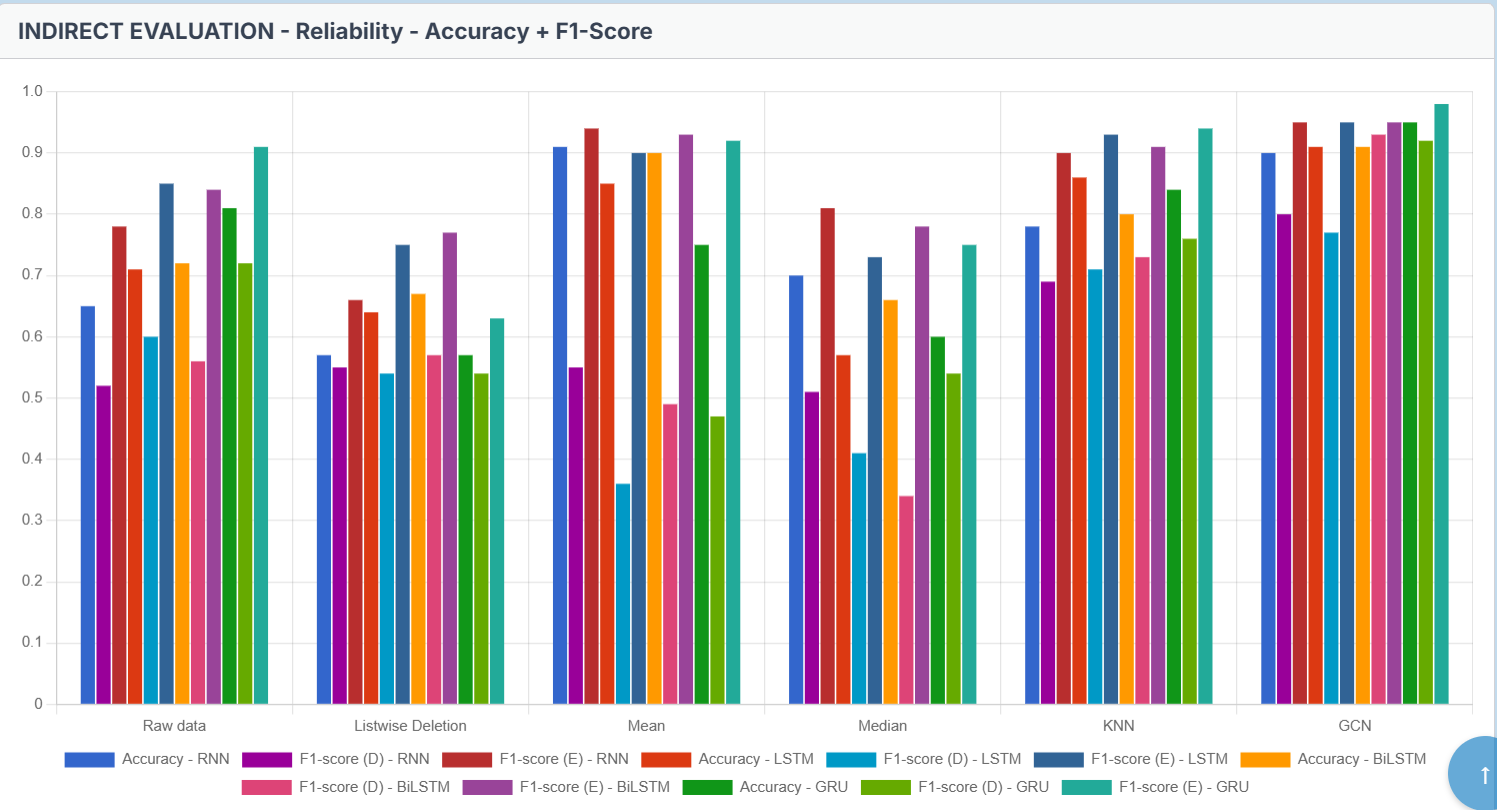
\includegraphics[width=\textwidth]{imgs/demo-indirect.png}
        \label{fig:sub1}
    \end{subfigure}
    \hfill
    \begin{subfigure}[b]{0.45\textwidth}
        \centering
        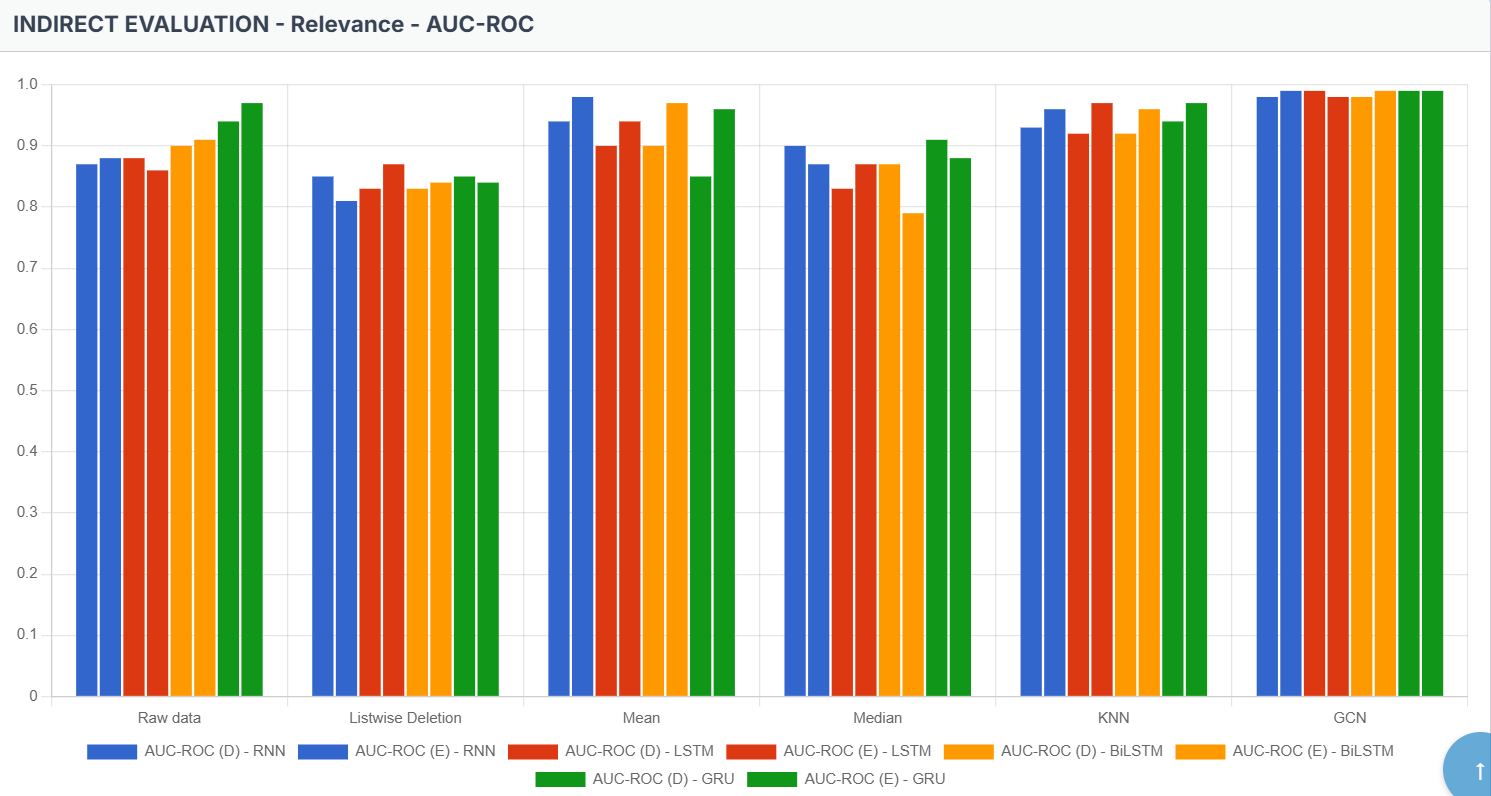
\includegraphics[width=\textwidth]{imgs/demo-indirect-aucroc.png}
        \label{fig:sub2}
    \end{subfigure}
    \caption{Kết quả đo lường chất lượng dữ liệu}
    \label{fig:2images}
\end{figure}


\subsection{Hiệu suất mô hình toàn diện}
\begin{figure}[H]
    \centering
    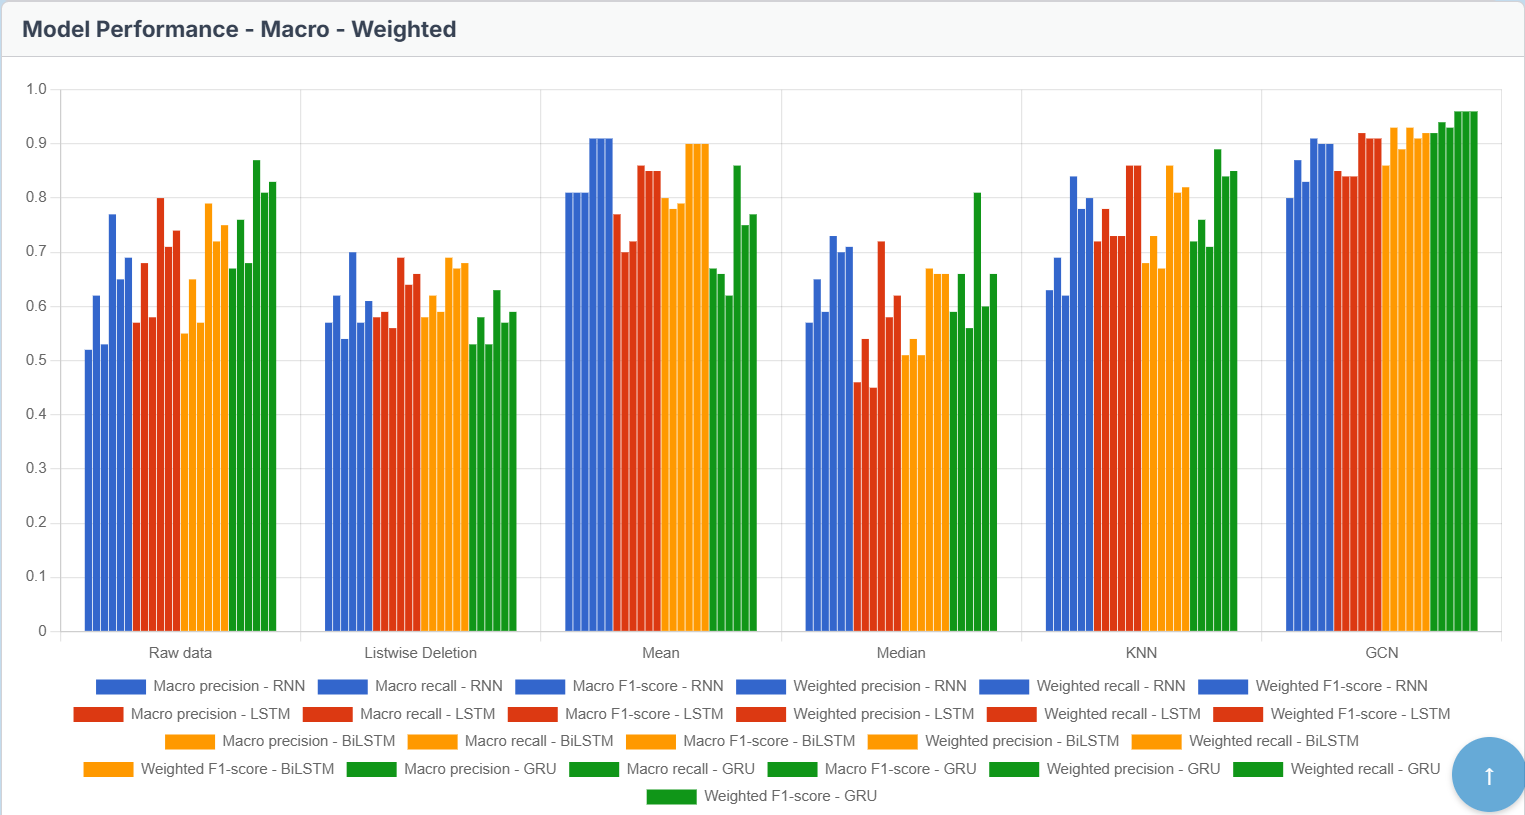
\includegraphics[width = 0.8\textwidth]{imgs/demo-modelperf.png}
    \caption{Biểu đồ so sánh hiệu suất mô hình qua các chỉ số Macro và Weighted}
    \label{fig:demo-modelperf}
\end{figure}

Ngoài ra, các chỉ số đánh giá mức độ trung bình là Macro và Weighted đã được sử dụng nhằm mang lại cái nhìn toàn diện và khách quan để đánh giá mô hình. Phương pháp điền khuyết bằng GCN do chúng tôi đề xuất đã mang lại sự cải thiện rõ rệt và ổn định trên tất cả các mô hình học sâu. Khi áp dụng GCN, mô hình GRU đạt được Macro F1-score cao nhất là 0.93 và Weighted F1-score là 0.96, vô cùng khả quan khi so sánh với các phương pháp khác. Ví dụ, với dữ liệu chưa xử lý, GRU chỉ đạt Macro F1-score tối đa 0.68, trong khi BiLSTM còn thấp hơn với 0.59 khi dùng phương pháp loại bỏ hàng bị thiếu. Ngay cả với các kỹ thuật điền khuyết phổ biến như Mean và KNN, kết quả vẫn chưa thể sánh bằng GCN. Cụ thể, Macro F1-score cao nhất của phương pháp Mean là 0.81 (RNN), còn KNN đạt 0.73 (LSTM). Trong khi đó, GCN luôn duy trì mức F1-score trên 0.83 với mọi mô hình được kiểm thử, cho thấy tính hiệu quả và độ ổn định vượt trội.

Sự vượt trội của GCN không chỉ nằm ở việc đạt được các điểm số cao nhất mà còn thể hiện ở tính ổn định và mạnh mẽ trên các kiến trúc mô hình khác nhau như RNN, LSTM, BiLSTM hay GRU.

\begin{sidewaystable}
\centering
\normalsize
\caption{Hiệu suất mô hình theo các chỉ số trung bình Macro và Weighted}
\renewcommand\arraystretch{2.8}
\label{tab:results-table}
\resizebox{\textheight}{!}{ % Mở rộng bảng theo chiều cao giấy
    \begin{tabular}{|c|c|c|c|c|c|c|c|c|c|c|c|c|c|c|c|c|c|c|c|c|c|c|c|c|}
        \hline
        \multirow{3}{*}{\textbf{Dataset}} & \multicolumn{12}{c|}{\textbf{Macro}} & \multicolumn{12}{c|}{\textbf{Weighted}} \\
        \cline{2-25}
        & \multicolumn{4}{c|}{\textbf{Macro Precision}} & \multicolumn{4}{c|}{\textbf{Macro Recall}} & \multicolumn{4}{c|}{\textbf{Macro F1-score}} & \multicolumn{4}{c|}{\textbf{Weighted Precision}} & 
        \multicolumn{4}{c|}{\textbf{Weighted Recall}} & 
        \multicolumn{4}{c|}{\textbf{Weighted F1-score}}\\
        \cline{2-25}
        & RNN &LSTM & BiLSTM & GRU & 
         RNN &LSTM & BiLSTM & GRU & 
          RNN &LSTM & BiLSTM & GRU & 
           RNN &LSTM & BiLSTM & GRU & 
            RNN &LSTM & BiLSTM & GRU & 
             RNN &LSTM & BiLSTM & GRU \\
        \cline{2-25}
        \hline
        Raw data & 0.52 & 0.57 & 0.55 & 0.67 & 0.62 & 0.68 & 0.65 & 0.76 & 0.53 & 0.58 & 0.57 & 0.68 & 0.77 & 0.80 & 0.79 & 0.87 & 0.65 & 0.71 & 0.72 & 0.81 & 0.69 & 0.74 & 0.75 & 0.83\\
        \hline
        Listwise Deletion & 0.57 & 0.58 & 0.58  & 0.53 & 0.62 & 0.59 & 0.62 & 0.58 & 0.54 & 0.56 & 0.59 & 0.53 & 0.70 & 0.69 & 0.69 & 0.63 & 0.57 & 0.64 & 0.67 & 0.57 & 0.61 & 0.66 & 0.68 & 0.59      \\
        \hline
        Mean & 0.81 & 0.77 & 0.80 & 0.67 & 0.81 & 0.70 & 0.78 & 0.66 & 0.81 & 0.72 & 0.79 & 0.62 & 0.91 & 0.86 & 0.90 & 0.86 & 0.91 & 0.85 & 0.90 & 0.75 & 0.91 & 0.85 & 0.90 & 0.77 \\
        \hline
        Median   & 0.57 & 0.46 & 0.51 & 0.59 & 0.65 & 0.54 & 0.54 & 0.66 & 0.59 & 0.45 & 0.51 & 0.56 & 0.73 & 0.72 & 0.67 & 0.81 & 0.70 & 0.57 & 0.66 & 0.60 & 0.71 & 0.62 & 0.66 & 0.66\\
        \hline
        KNN  & 0.63 & 0.72 & 0.68 & 0.72 & 0.69 & 0.78 & 0.73 & 0.76 & 0.62 & 0.73 & 0.67 & 0.71 & 0.84 & 0.73 & 0.86 & 0.89 & 0.78 & 0.86 & 0.81 & 0.84 & 0.80 & 0.86 & 0.82 & 0.85 \\
        \hline
        KI  & 0.53 & 0.82 & 0.57 & 0.80 & 0.63 & 0.71 & 0.65 & 0.76 & 0.56 & 0.62 & 0.58 & 0.77 & 0.78 & 0.82 & 0.80 & 0.80 & 0.72 & 0.75 & 0.73 & 0.75 & 0.74 & 0.78 & 0.75 & 0.76 \\
        \hline
        \textbf{GCN}  & \textbf{0.80} & \textbf{0.85} & \textbf{0.86} & \textbf{0.92} & \textbf{0.87} & \textbf{0.84} & \textbf{0.93} & \textbf{0.94} & \textbf{0.83} & \textbf{0.84} & \textbf{0.89} & \textbf{0.93} & \textbf{0.91} & \textbf{0.92} & \textbf{0.93} & \textbf{0.96} & \textbf{0.90} & \textbf{0.91} & \textbf{0.91} &
        \textbf{0.96} & \textbf{0.90} & \textbf{0.91} & \textbf{0.92} & \textbf{0.96}  \\
        \hline
    \end{tabular}
}
\end{sidewaystable}



% \renewcommand\arraystretch{2.8}
% \begin{sidewaystable} 
% \centering
% \normalsize
% \caption{So sánh hiệu quả phương pháp điền khuyết KI vs GCN-I}
% \label{tab:results-table-quality-knn-gcn}
% \resizebox{\textheight}{!}{
%     \begin{tabular}{|c|c|c|c|c|c|c|c|c|c|c|c|c|c|c|c|c|c|c|c|c|c|c|}
%         \hline
%         \multirow{4}{*}{\textbf{Dataset}} & \multicolumn{2}{c|}{\textbf{Direct Evaluation}} & \multicolumn{20}{c|}{\textbf{Indirect Evaluation}} \\
%         \cline{2-23}
%         & \multirow{2}{*}{\textbf{Completeness}} & \multirow{2}{*}{\textbf{Consistency}} & \multicolumn{12}{c|}{\textbf{Reliability}} & \multicolumn{8}{c|}{\textbf{Relevance}}\\
%         \cline{4-23}
%         & & &\multicolumn{4}{c|}{Accuracy} & \multicolumn{8}{c|}{F1-Score} & \multicolumn{8}{c|}{AUC-ROC} \\
%         \cline{4-23}
%         & & & \multirow{2}{*} {RNN} & \multirow{2}{*} {LSTM} & \multirow{2}{*} {BiLSTM} & \multirow{2}{*} {GRU} & \multicolumn{4}{c|}{Label D} & \multicolumn{4}{c|}{Label E} & \multicolumn{4}{c|}{Label D} & \multicolumn{4}{c|}{Label E}\\ 
%         \cline{8-23}
%         & & & &  & & & RNN & LSTM & BiLSTM & GRU & RNN & LSTM & BiLSTM & GRU & RNN & LSTM & BiLSTM & GRU & RNN & LSTM & BiLSTM & GRU \\
%         \cline{7-23}
%         \hline
%         KI  & 100\% & 99.77\% & 0.72 & 0.76 & 0.73 & 0.75 & 0.56 & 0.60 & 0.57 & 0.62 & 0.85 & 0.87 & 0.86 & 0.86 & 0.87 & 0.89 & 0.90 & 0.87 & 0.91 & 0.92 & 0.91 & 0.91 \\
%         \hline
%         \textbf{GCN}  & 100\% & 100\% & \textbf{0.90} & \textbf{0.91} & \textbf{0.91} & \textbf{0.95} & \textbf{0.80} & \textbf{0.77} & \textbf{0.93} & \textbf{0.92} & \textbf{0.95} & \textbf{0.95} & \textbf{0.95} & \textbf{0.98} & \textbf{0.99} & \textbf{0.98} & \textbf{0.99} & \textbf{0.99} & \textbf{0.98} & \textbf{0.98} & \textbf{0.99} & \textbf{0.99}  \\
%         \hline
%     \end{tabular}
% }
% \end{sidewaystable}


% \begin{sidewaystable}
% \centering
% \normalsize
% \caption{Hiệu suất mô hình theo các chỉ số trung bình Macro và Weighted của phương pháp KI vs GCN-I}
% \renewcommand\arraystretch{2.8}
% \label{tab:results-table-knn-gcn}
% \resizebox{\textheight}{!}{
%     \begin{tabular}{|c|c|c|c|c|c|c|c|c|c|c|c|c|c|c|c|c|c|c|c|c|c|c|c|c|}
%         \hline
%         \multirow{3}{*}{\textbf{Dataset}} & \multicolumn{12}{c|}{\textbf{Macro}} & \multicolumn{12}{c|}{\textbf{Weighted}} \\
%         \cline{2-25}
%         & \multicolumn{4}{c|}{\textbf{Macro Precision}} & \multicolumn{4}{c|}{\textbf{Macro Recall}} & \multicolumn{4}{c|}{\textbf{Macro F1-score}} & \multicolumn{4}{c|}{\textbf{Weighted Precision}} & 
%         \multicolumn{4}{c|}{\textbf{Weighted Recall}} & 
%         \multicolumn{4}{c|}{\textbf{Weighted F1-score}}\\
%         \cline{2-25}
%         & RNN &LSTM & BiLSTM & GRU & 
%          RNN &LSTM & BiLSTM & GRU & 
%           RNN &LSTM & BiLSTM & GRU & 
%            RNN &LSTM & BiLSTM & GRU & 
%             RNN &LSTM & BiLSTM & GRU & 
%              RNN &LSTM & BiLSTM & GRU \\
%         \cline{2-25}
%         \hline
%         KI  & 0.53 & 0.82 & 0.57 & 0.80 & 0.63 & 0.71 & 0.65 & 0.76 & 0.56 & 0.62 & 0.58 & 0.77 & 0.78 & 0.82 & 0.80 & 0.80 & 0.72 & 0.75 & 0.73 & 0.75 & 0.74 & 0.78 & 0.75 & 0.76 \\
%         \hline
%         \textbf{GCN}  & \textbf{0.80} & \textbf{0.85} & \textbf{0.86} & \textbf{0.92} & \textbf{0.87} & \textbf{0.84} & \textbf{0.93} & \textbf{0.94} & \textbf{0.83} & \textbf{0.84} & \textbf{0.89} & \textbf{0.93} & \textbf{0.91} & \textbf{0.92} & \textbf{0.93} & \textbf{0.96} & \textbf{0.90} & \textbf{0.91} & \textbf{0.91} &
%         \textbf{0.96} & \textbf{0.90} & \textbf{0.91} & \textbf{0.92} & \textbf{0.96}  \\
%         \hline
%     \end{tabular}
% }
% \end{sidewaystable}


